
%\begin{center}

      \pagestyle{empty}


~

\vspace{-5mm}

\hspace{-9mm}
\framebox[1.05\width]{

  \begin{minipage}[t][25cm]{16cm}  %% 24 cm
  \rule{0cm}{5mm}

  \vspace{-.3cm}
  \large  \hfill Note C-AD/AP/470 (BNL, Oct. 2012) \\[-.5cm]

  \vfill
  \vspace{-2cm}
  \title{ 
      \textbf{
              \huge ZGOUBI USERS' GUIDE     \\
                  ~                          \\
              \large ZGOUBI ON WEB~: \\ http://sourceforge.net/projects/zgoubi/
             }    
        }

    \author{ 
             \textbf{Fran\c{c}ois M\'eot }                      \\[0ex]
             { \em Brookhaven National Laboratory   }             \\[-.9ex]
             {\em Collider-Accelerator Department   }            \\[-.9ex]
             { \em Upton, NY, 11973 }           
           }

    \maketitle

  \vfill  %space{2cm}

    \date

    \vfill


      { \hspace{15mm} ATLAS \& CMS IRs, LHC \hspace{35mm}  Snake Resonance Crossing, RHIC \hfill } \\[1ex]
    %
    \centerline{
      \mbox{\hspace{-3ex}
         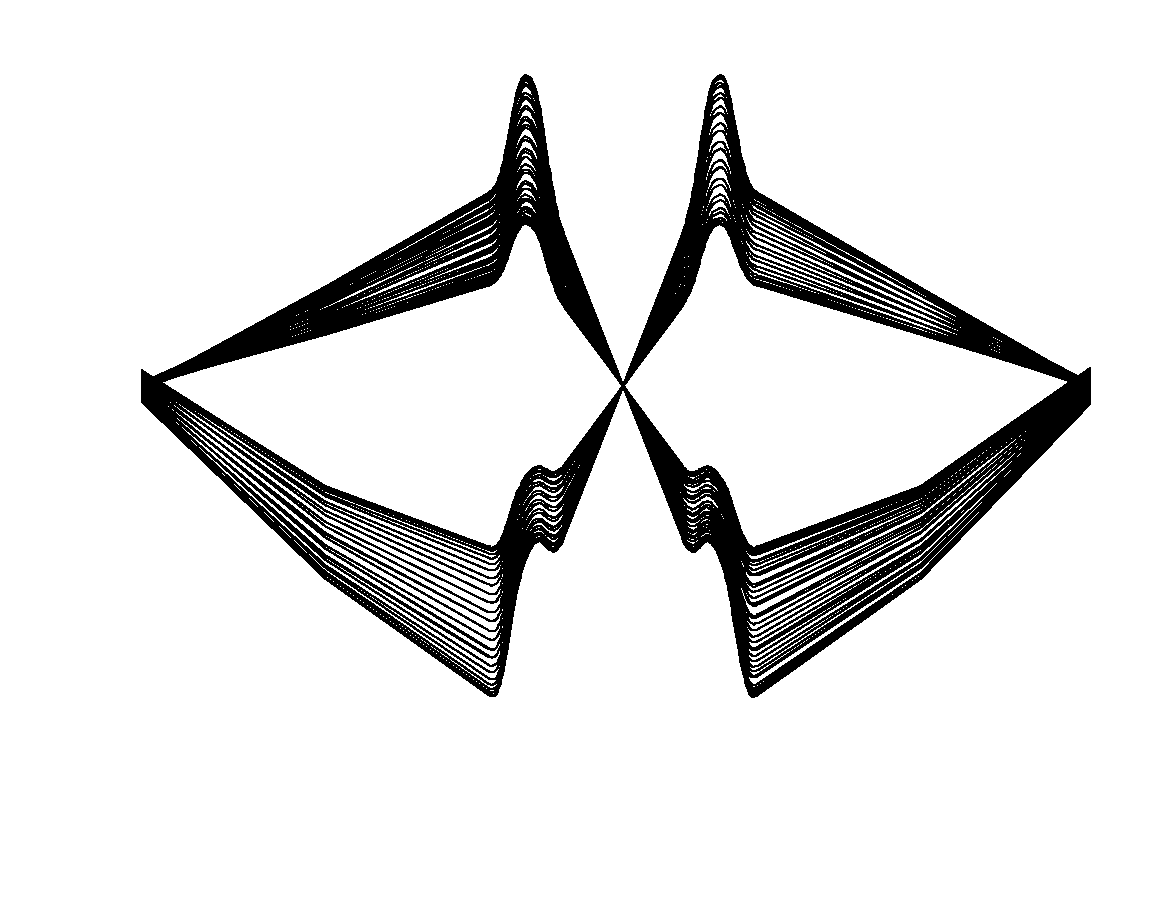
\includegraphics[width=10cm]{FigCover1.ps}
          \hspace{5ex}
         \includegraphics[width=9cm,height=5cm]{FigCover2New.ps} 
       }
     }


      {  \hspace{3mm} Spin flip during ramp, AGS with snakes \hspace{22mm} ~ ~ Serpentine acceleration, EMMA \hfill } \\[1.2ex]
     %
    \centerline{
      \mbox{\hspace{-1ex}
         \hspace{0mm}
         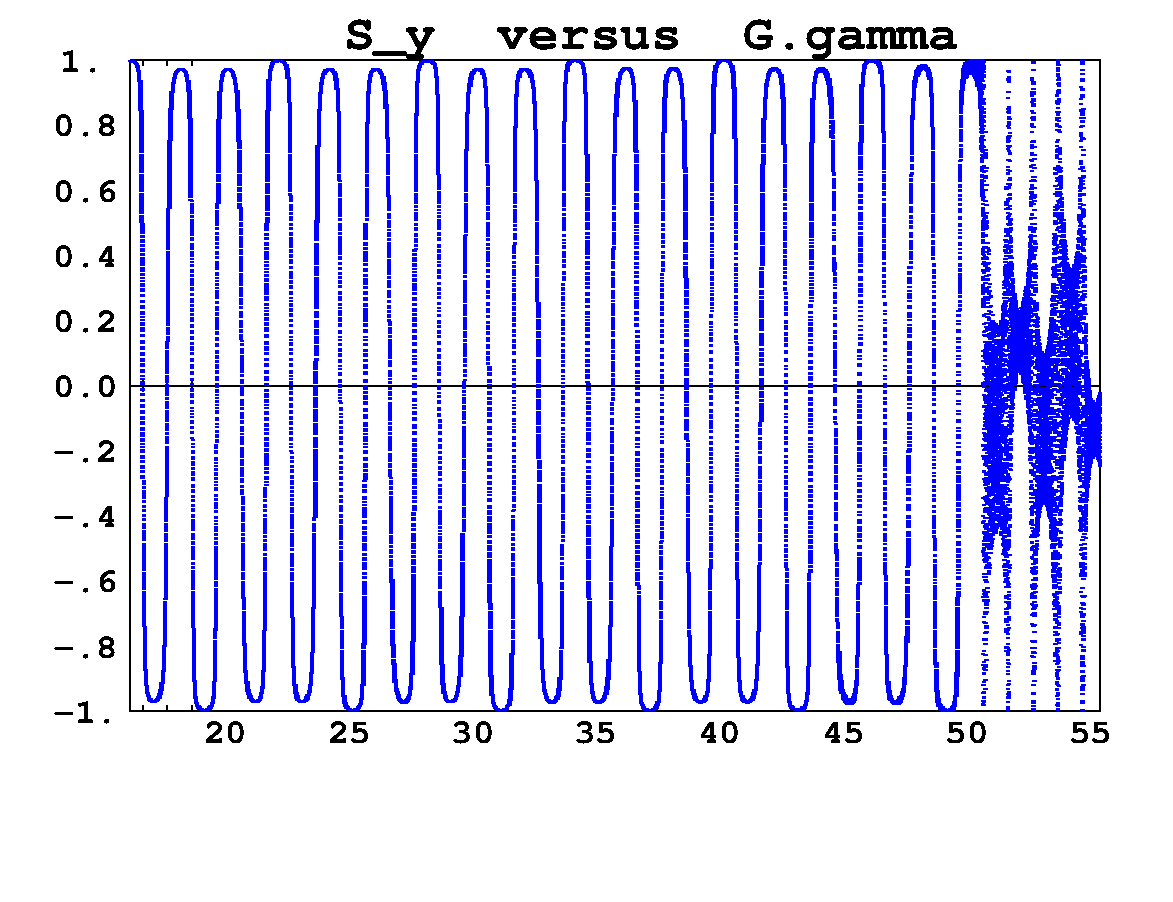
\includegraphics[width=7.2cm,height=4.cm]{FigCover3New.ps}
         \hspace{9ex}
%         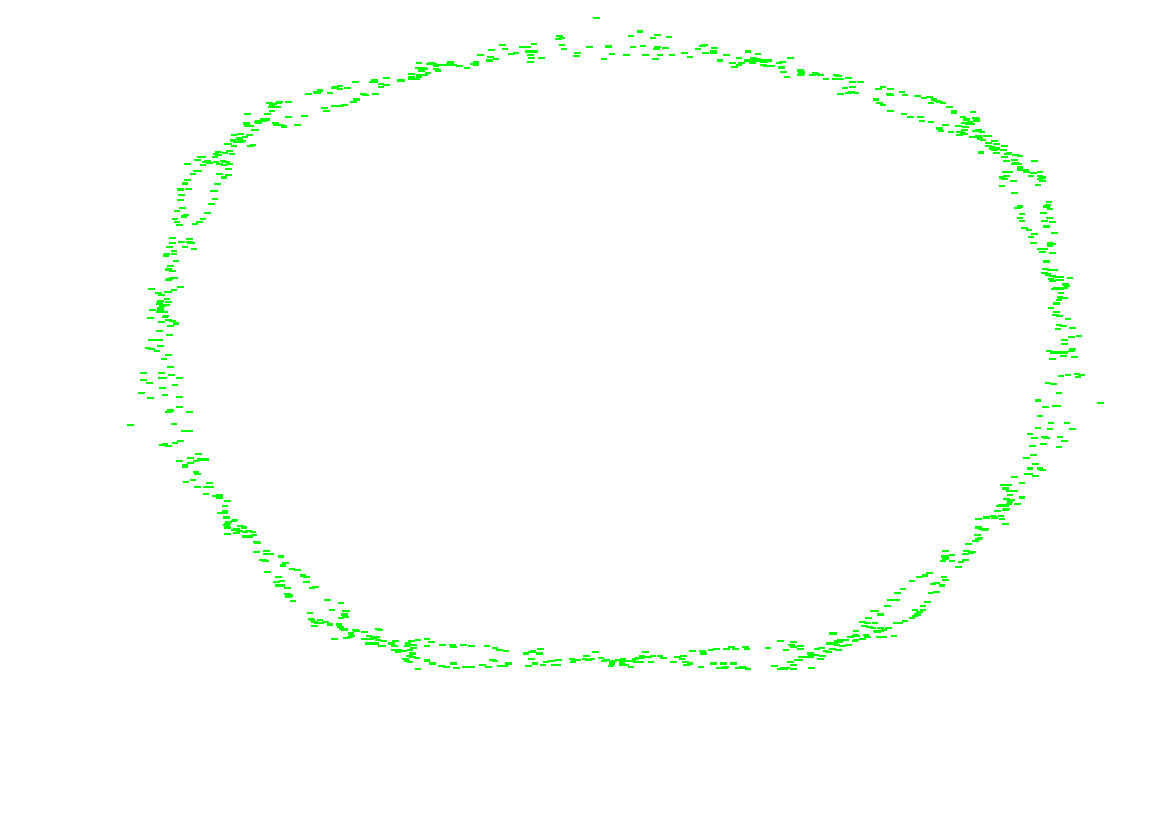
\includegraphics[width=7cm]{FigCover4.ps}
         \includegraphics[bbllx=20,bblly=30,bburx=567,bbury=440,width=7cm]{FigCover4_New.ps}
       }
     }

  \end{minipage}
}
%\end{center}


\newpage


~~~~~~~~~~~
  \footnotetext{\Large  {\bf Cover figures} :  \\
  {\it upper left}~: collision optics at ATLAS and CMS~\cite{LHCb10}, \\
  {\it upper right}~: polarization upon crossing of 393+$Q_y$ resonance in RHIC~\cite{polarRHIC},  \\
  {\it lower left}~: spin-flip cycle in the AGS with helical snakes~\cite{polarAGS},   \\
  {\it lower right}~: serpentine acceleration in the prototype linear FFAG EMMA~\cite{repDapniaEMMA,EMMA}. 
   }

